\documentclass[11pt,a4paper]{article}

% ==============================================================================
% PACKAGES & GEOMETRY SETTINGS (Guarantees zero overflow, crisp formatting)
% ==============================================================================
\usepackage[a4paper,top=2.2cm,bottom=2.2cm,left=2.2cm,right=2.2cm]{geometry}
\usepackage[utf8]{inputenc}
\usepackage[T1]{fontenc}
\usepackage{lmodern}
\usepackage{microtype}
\usepackage{amsmath,amssymb,amsfonts}
\usepackage{booktabs}
\usepackage{tabularx}
\usepackage{array}
\usepackage{enumitem}
\usepackage{xcolor}
\usepackage{tikz}
\usetikzlibrary{shapes.geometric, arrows.meta, positioning, fit, backgrounds, calc}
\usepackage{tcolorbox}
\tcbuselibrary{skins,breakable}
\usepackage{fancyhdr}
\usepackage{titlesec}
\usepackage{caption}
\usepackage{float}
\usepackage{hyperref}

% ==============================================================================
% COLOR PALETTE (Modern Corporate / Academic Deep Navy & Slate)
% ==============================================================================
\definecolor{primarynavy}{RGB}{20, 35, 75}
\definecolor{accentteal}{RGB}{0, 128, 128}
\definecolor{darkslate}{RGB}{45, 55, 72}
\definecolor{lightgreybg}{RGB}{248, 249, 252}
\definecolor{bordergrey}{RGB}{226, 232, 240}
\definecolor{crimsonred}{RGB}{180, 40, 40}
\definecolor{forestgreen}{RGB}{34, 139, 34}

% ==============================================================================
% HYPERLINK SETUP
% ==============================================================================
\hypersetup{
    colorlinks=true,
    linkcolor=primarynavy,
    citecolor=accentteal,
    urlcolor=accentteal,
    pdfauthor={Vedant Panchal (23AIML042), Dax Virani (23AIML076)},
    pdftitle={MIRAGE: Autonomous Multimodal Hallucination Detection & Factual Verification System},
    pdfsubject={Project Approval Report - CSPIT AIML}
}

% ==============================================================================
% SECTION FORMATTING & HEADERS
% ==============================================================================
\titleformat{\section}
  {\color{primarynavy}\normalfont\Large\bfseries}{\thesection}{1em}{}[\titlerule]
\titleformat{\subsection}
  {\color{accentteal}\normalfont\large\bfseries}{\thesubsection}{1em}{}
\titleformat{\subsubsection}
  {\color{darkslate}\normalfont\normalsize\bfseries}{\thesubsubsection}{1em}{}

\pagestyle{fancy}
\fancyhf{}
\renewcommand{\headrulewidth}{0.4pt}
\renewcommand{\footrulewidth}{0.4pt}
\fancyhead[L]{\small\color{darkslate}\textbf{MIRAGE Project Proposal}}
\fancyhead[R]{\small\color{darkslate}CSPIT --- Dept. of AI \& ML}
\fancyfoot[L]{\small\color{darkslate}Vedant (23AIML042) \& Dax (23AIML076)}
\fancyfoot[R]{\small\color{darkslate}Page \thepage}

% ==============================================================================
% CUSTOM CALLOUT BOXES
% ==============================================================================
\newtcolorbox{calloutbox}[2][]{
    enhanced,
    colback=lightgreybg,
    colframe=primarynavy,
    coltitle=white,
    fonttitle=\bfseries,
    title=#2,
    arc=3mm,
    boxrule=1pt,
    left=4mm,right=4mm,top=3mm,bottom=3mm,
    #1
}

\newtcolorbox{analogybox}[2][]{
    enhanced,
    colback=white,
    colframe=accentteal,
    coltitle=white,
    fonttitle=\bfseries,
    title=#2,
    arc=3mm,
    boxrule=1pt,
    left=4mm,right=4mm,top=3mm,bottom=3mm,
    #1
}

\newtcolorbox{alertbox}[2][]{
    enhanced,
    colback=white,
    colframe=crimsonred,
    coltitle=white,
    fonttitle=\bfseries,
    title=#2,
    arc=3mm,
    boxrule=1pt,
    left=4mm,right=4mm,top=3mm,bottom=3mm,
    #1
}

% ==============================================================================
% DOCUMENT BEGIN
% ==============================================================================
\begin{document}

% ------------------------------------------------------------------------------
% TITLE BLOCK & ACADEMIC AFFILIATION
% ------------------------------------------------------------------------------
\begin{titlepage}
    \centering
    \vspace*{0.5cm}
    
    {\Large\scshape Chandubhai S. Patel Institute of Technology (CSPIT)\par}
    \vspace{0.2cm}
    {\large\scshape Department of Artificial Intelligence and Machine Learning\par}
    \vspace{0.8cm}
    
    \rule{\linewidth}{1.5pt}\\[0.4cm]
    {\huge\bfseries\color{primarynavy} PROJECT APPROVAL REPORT\\[0.3cm]}
    {\Large\bfseries\color{accentteal} MIRAGE: Autonomous Multimodal Hallucination Detection \& Factual Consistency Verification System for Production LLMs\par}
    \rule{\linewidth}{1.5pt}\\[1.2cm]
    
    \begin{tcolorbox}[colback=lightgreybg,colframe=primarynavy,arc=2mm,boxrule=1pt,width=0.92\linewidth]
        \centering
        \textbf{\large Project Metadata \& Student Credentials}\\[0.2cm]
        \begin{tabular}{ll}
            \textbf{Student Name 1:} & Vedant Panchal \quad (\textbf{Roll No:} 23AIML042) \\
            \textbf{Student Name 2:} & Dax Virani \quad (\textbf{Roll No:} 23AIML076) \\
            \textbf{Degree Program:} & Bachelor of Technology in Artificial Intelligence \& ML \\
            \textbf{Institution:}    & Chandubhai S. Patel Institute of Technology \\
            \textbf{Academic Year:}  & 2026--2027 \\
            \textbf{Project Track:}  & Enterprise AI Systems, Safe Autonomy \& Robust LLMs \\
            \textbf{Project Status:} & Architectural Implementation Phase (P0 Complete, P1 Initiated)
        \end{tabular}
    \end{tcolorbox}
    
    \vspace{1.2cm}
    
    \begin{abstract}
    \noindent Large Language Models (LLMs) suffer from \textit{hallucinations}---generating confident, grammatically persuasive statements that are factually incorrect, unsupported by evidence, or self-contradictory. In high-stakes production domains such as healthcare, finance, and legal compliance, uncalibrated hallucinations cause severe real-world harm. \textbf{MIRAGE} is an autonomous, black-box middleware platform that intercepts LLM completions in real time, evaluates them across a parallel five-signal verification pipeline (Retrieval-Augmented Verification, Self-Consistency Sampling with Semantic Entropy, DeBERTa NLI Entailment, LLaVA Visual Grounding, and Intra-Response Internal Consistency), computes a statistically calibrated \textbf{Hallucination Risk Score (HRS)} with Mondrian Conformal Prediction bounds, and autonomously rewrites contradicted claims via a self-healing agentic correction loop before the response reaches the end user. This proposal details the problem statement, product taxonomy, architectural design, mathematical foundations, and implementation feasibility for faculty evaluation and project approval.
    \end{abstract}
    
    \vfill
    {\small\color{darkslate}\textbf{Keywords:} Large Language Models, Hallucination Detection, Conformal Prediction, Natural Language Inference, Multi-Signal Verification, AI Safety, Microservices Middleware.}
\end{titlepage}

\newpage
\tableofcontents
\newpage

% ==============================================================================
% SECTION 1: PROBLEM STATEMENT & MOTIVATION
% ==============================================================================
\section{Problem Statement (PS) and Industry Motivation}

\subsection{The Hallucination Crisis in Production Generative AI}
Generative Large Language Models (e.g., GPT-4o, Llama 3.1, Claude 3.5, Mixtral) have revolutionized text generation, code synthesis, and analytical question answering. However, by their fundamental mathematical formulation, LLMs are autoregressive probability distributions over token sequences:
\begin{equation}
P(w_1, w_2, \dots, w_T) = \prod_{t=1}^T P(w_t \mid w_1, w_2, \dots, w_{t-1})
\end{equation}
They optimize for \textbf{token likelihood}, \textit{not} truthfulness, epistemic validity, or verifiable factual evidence. Consequently, LLMs exhibit \textbf{hallucinations}---generating outputs that appear coherent, structured, and authoritative, yet are completely fabricated or contrary to known facts.

\begin{alertbox}{Real-World Failures Caused by LLM Hallucinations}
\begin{itemize}[leftmargin=*]
    \item \textbf{Clinical \& Healthcare:} An LLM prescribed a contraindicated dosage of Metformin alongside an incompatible antibiotic because both occurred frequently in disparate medical training sets, creating lethal clinical risk.
    \item \textbf{Legal Practice:} An attorney submitted an LLM-generated brief citing fictional legal cases (\textit{Mata v. Avianca}), leading to judicial sanctions and professional disbarment.
    \item \textbf{Financial Advising:} An enterprise financial bot hallucinated a 42\% revenue growth metric for a competitor by conflating two separate quarterly reporting tables, distorting multi-million dollar investment strategies.
    \item \textbf{Customer Operations:} An e-commerce chatbot promised a customer an unauthorized 100\% cash refund citing a nonexistent internal corporate warranty clause, forcing the firm to honour the dispute in small-claims court.
\end{itemize}
\end{alertbox}

\subsection{Why Existing Solutions Fail}
Current industrial approaches to hallucination mitigation suffer from four fundamental limitations:
\begin{enumerate}[leftmargin=*]
    \item \textbf{Naive Prompt Engineering (``Think step-by-step'' / System Prompts):} LLMs still hallucinate within chain-of-thought traces, often inventing plausible justifications for false claims.
    \item \textbf{Standard Retrieval-Augmented Generation (RAG) Alone:} Standard RAG retrieves documents, but LLMs frequently ignore retrieved context, misinterpret retrieved numbers, or introduce hallucinations outside the context window.
    \item \textbf{LLM-as-a-Judge:} Using a second LLM (e.g., GPT-4) to grade the first model is prohibitively expensive, introduces $3\times$ to $5\times$ latency, and suffers from correlated errors where both models hallucinate on the exact same subtle prompts.
    \item \textbf{Uncalibrated Binary Outputs:} Existing security tools return a simplistic ``True/False'' flag without statistical uncertainty bounds. In enterprise compliance, a risk score of $0.82$ must mathematically mean an \textit{82\% empirical probability of factual error}.
\end{enumerate}

\subsection{Formal Problem Statement}
\begin{tcolorbox}[colback=lightgreybg,colframe=primarynavy,title=\textbf{Formal Academic Problem Statement}]
\textit{``To design, implement, and benchmark an autonomous, zero-modification middleware system that intercepts multimodal LLM responses, decomposes them into atomic factual assertions, evaluates them concurrently across independent retrieval, semantic dispersion, entailment, visual, and internal consistency signals, and synthesizes a calibrated Hallucination Risk Score (HRS) with distribution-free conformal prediction bounds, while autonomously repairing contradicted claims under a sub-3-second end-to-end latency constraint.''}
\end{tcolorbox}

% ==============================================================================
% SECTION 2: NON-TECHNICAL OVERVIEW & ANALOGY
% ==============================================================================
\section{Non-Technical Overview: The Plain-English Analogy}

To understand MIRAGE without a machine learning background, consider how reputable newspaper publishing and courtroom journalism operate in the real world.

\begin{analogybox}{The Analogy: The Overconfident Reporter vs. The Chief Fact-Checking Desk}
Imagine you run a premier international newspaper. You have hired a brilliant, lightning-fast junior reporter named \textbf{``Alex''} (representing any modern LLM like GPT-4 or Llama). 
\begin{itemize}[leftmargin=*]
    \item \textbf{Alex's Superpower:} Alex can write a 2,000-word article on quantum physics, French history, or corporate earnings in 2 seconds flat, with gorgeous prose, eloquent metaphors, and perfect grammar.
    \item \textbf{Alex's Dangerous Flaw:} Alex possesses zero self-doubt. When Alex forgets a detail---like the exact date a company was founded or the capital city of an obscure territory---Alex does not say \textit{``I don't know.''} Instead, Alex invents a realistic-sounding fact out of thin air with 100\% confidence!
    \item \textbf{The Disaster Scenario:} If the newspaper prints Alex's drafts directly onto the front page without inspection, the newspaper faces defamation lawsuits, loss of journalistic credibility, and disaster.
\end{itemize}
\textbf{How MIRAGE Solves This:}
MIRAGE acts as the \textbf{Chief Fact-Checking Desk} seated directly between Alex and the printing press:
\begin{enumerate}
    \item \textbf{The Decomposer (The Line Editor):} Breaks Alex's story down sentence by sentence into atomic checkable claims (e.g., Claim 1: \textit{``Company was founded in 2012''}, Claim 2: \textit{``Revenue reached \$50M''}).
    \item \textbf{Signal 1: The Library Archive (RAV):} Searches the company's verified encyclopedia and database to see if records confirm the claim.
    \item \textbf{Signal 2: The Interrogation Room (SCS):} Asks Alex the same question 5 times in different ways. If Alex gives 5 wildly different answers, Alex is guessing!
    \item \textbf{Signal 3: The Cross-Examiner (NLI):} Takes the verified library records and strictly checks: \textit{``Does document A prove statement B, or does it contradict it?''}
    \item \textbf{Signal 4: The Photo Inspector (Visual Grounding):} If Alex claims a photo shows a red Ferrari, checks the referenced image to confirm whether it is actually a red Ferrari.
    \item \textbf{Signal 5: The Logic Auditor (Internal Consistency):} Checks if Alex contradicted himself (e.g., saying the CEO was born in 1980 on page 1, but graduated college in 1985 on page 2).
    \item \textbf{The Risk Calculator (HRS):} Combines all evidence into a single, calibrated risk rating (Low, Medium, High, or Critical).
    \item \textbf{The Red Pen Editor (Agentic Correction):} If the risk is High, the desk does not discard the story or crash the system; it takes a red pen, strikes out the false sentence, rewrites it accurately using verified archive facts, and sends the polished, truth-verified story to the reader.
\end{enumerate}
\end{analogybox}

% ==============================================================================
% SECTION 3: PRODUCT TAXONOMY & BREAKDOWN
% ==============================================================================
\section{Product Taxonomy: What Kind of Product Are We Building?}

When evaluating an applied engineering capstone or research system, faculty frequently ask: \textit{``Is this an API, a website, a mobile application, an MCP server, or a standalone ML model?''}

\textbf{MIRAGE is an Enterprise AI Safety Middleware Platform} comprising five interconnected product interfaces:

\begin{table}[H]
\centering
\small
\renewcommand{\arraystretch}{1.3}
\begin{tabularx}{\linewidth}{p{3.2cm} p{3.2cm} X}
\toprule
\textbf{Product Interface} & \textbf{Target Consumer} & \textbf{Product Role \& Engineering Implementation} \\
\midrule
\textbf{1. Drop-in REST Proxy API} & Enterprise Software Engineers \& Backend Apps & High-performance FastAPI reverse proxy (\texttt{/v1/chat/completions}) compatible with OpenAI, Groq, OpenRouter, and Anthropic. Applications redirect their base URL to MIRAGE with \textbf{zero code rewrites}. \\
\textbf{2. Direct Verification REST API} & Workflow Orchestrators \& Pipeline Integrations & Dedicated endpoint (\texttt{POST /v1/verify}) where applications send pre-generated (\texttt{prompt}, \texttt{response}) pairs and receive full calibrated claim breakdowns and risk scores. \\
\textbf{3. Real-Time Streaming WebSocket} & Interactive Chatbots \& UI Applications & Bidirectional persistent WebSocket (\texttt{/v1/verify/stream}) providing incremental, token-by-token verification events as the LLM generates output. \\
\textbf{4. Model Context Protocol (MCP) Server} & AI IDEs, Cursor, Claude Desktop, Copilot & Standardized MCP server exposing \texttt{check\_hallucination}, \texttt{verify\_factual\_consistency}, and \texttt{get\_health\_status} tools to autonomous agents. \\
\textbf{5. Longitudinal Drift Web Dashboard (Site)} & AI Safety Officers, Operators, Compliance & Production React 18 / Vite web application displaying longitudinal Population Stability Index (PSI) drift trends, TreeSHAP waterfall charts, claim trees, and PDF audit certificates. \\
\bottomrule
\end{tabularx}
\caption{Taxonomy of MIRAGE Product Interfaces and Deployment Targets.}
\label{tab:product_taxonomy}
\end{table}

% ==============================================================================
% SECTION 4: HOW OUR SYSTEM WORKS (SYSTEM WORKFLOW)
% ==============================================================================
\section{How the System Works: End-to-End Execution Flow}

\begin{figure}[H]
\centering
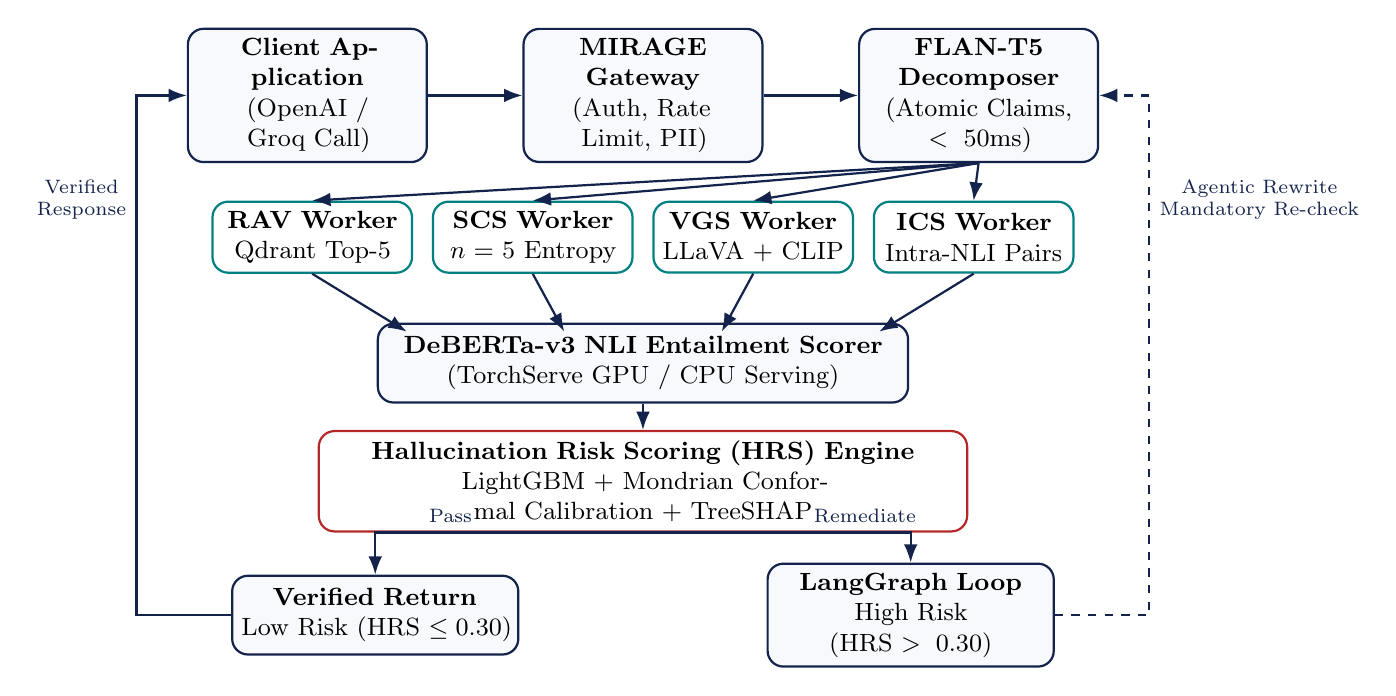
\begin{tikzpicture}[
    node distance=1.1cm and 0.8cm,
    every node/.style={font=\small},
    box/.style={rectangle, rounded corners=2mm, draw=primarynavy, fill=lightgreybg, thick, text width=2.8cm, align=center, minimum height=1cm},
    worker/.style={rectangle, rounded corners=2mm, draw=accentteal, fill=white, thick, text width=2.3cm, align=center, minimum height=0.9cm},
    engine/.style={rectangle, rounded corners=2mm, draw=crimsonred, fill=white, thick, text width=3.2cm, align=center, minimum height=1cm},
    arrow/.style={-Latex, thick, color=primarynavy}
]

% Row 1: Ingestion & Decomposition (Centered)
\node[box] (gw) at (0, 0) {\textbf{MIRAGE Gateway}\\(Auth, Rate Limit, PII)};
\node[box, left=1.2cm of gw] (app) {\textbf{Client Application}\\(OpenAI / Groq Call)};
\node[box, right=1.2cm of gw] (decom) {\textbf{FLAN-T5 Decomposer}\\(Atomic Claims, $<50$ms)};

% Row 2: Multi-Signal Workers (Symmetrically distributed)
\node[worker] (rav) at (-4.2, -1.8) {\textbf{RAV Worker}\\Qdrant Top-5};
\node[worker] (scs) at (-1.4, -1.8) {\textbf{SCS Worker}\\$n=5$ Entropy};
\node[worker] (vgs) at (1.4, -1.8) {\textbf{VGS Worker}\\LLaVA + CLIP};
\node[worker] (ics) at (4.2, -1.8) {\textbf{ICS Worker}\\Intra-NLI Pairs};

% Row 3: NLI Scorer (Centered)
\node[box, text width=6.5cm] (nli) at (0, -3.4) {\textbf{DeBERTa-v3 NLI Entailment Scorer}\\(TorchServe GPU / CPU Serving)};

% Row 4: HRS Engine (Centered)
\node[engine, text width=8.0cm] (hrs) at (0, -4.9) {\textbf{Hallucination Risk Scoring (HRS) Engine}\\LightGBM + Mondrian Conformal Calibration + TreeSHAP};

% Row 5: Decision & Routing
\node[box, text width=3.4cm] (pass) at (-3.4, -6.6) {\textbf{Verified Return}\\Low Risk (HRS $\le 0.30$)};
\node[box, text width=3.4cm] (correct) at (3.4, -6.6) {\textbf{LangGraph Loop}\\High Risk (HRS $> 0.30$)};

% Arrows
\draw[arrow] (app) -- (gw);
\draw[arrow] (gw) -- (decom);

% Decomposer to 4 Workers
\draw[arrow] (decom.south) -- (rav.north);
\draw[arrow] (decom.south) -- (scs.north);
\draw[arrow] (decom.south) -- (vgs.north);
\draw[arrow] (decom.south) -- (ics.north);

% Workers to NLI Scorer
\draw[arrow] (rav.south) -- (-3.0, -3.0);
\draw[arrow] (scs.south) -- (-1.0, -3.0);
\draw[arrow] (vgs.south) -- (1.0, -3.0);
\draw[arrow] (ics.south) -- (3.0, -3.0);

% NLI to HRS
\draw[arrow] (nli) -- (hrs);

% HRS to Branches
\draw[arrow] (hrs.south) -| (pass.north) node[pos=0.3, above left, font=\scriptsize] {Pass};
\draw[arrow] (hrs.south) -| (correct.north) node[pos=0.3, above right, font=\scriptsize] {Remediate};

% Safe Return Loop (Clear of all boxes along left margin)
\draw[arrow] (pass.west) -- ++(-1.2, 0) |- node[pos=0.4, left, font=\scriptsize, align=center] {Verified\\Response} (app.west);

% Rewrite Feedback Loop (Clear of all boxes along right margin)
\draw[arrow, dashed] (correct.east) -- ++(1.2, 0) |- node[pos=0.4, right, font=\scriptsize, align=center] {Agentic Rewrite\\Mandatory Re-check} (decom.east);

\end{tikzpicture}
\caption{End-to-End High-Level Execution Pipeline of the MIRAGE Middleware.}
\label{fig:high_level_pipeline}
\end{figure}

The verification lifecycle follows six rigorous stages:
\begin{enumerate}[leftmargin=*]
    \item \textbf{Interception \& Authentication:} The client application dispatches an OpenAI-formatted payload. The MIRAGE Gateway validates the cryptographic tenant API key / JWT, scrubs spoofed headers (\texttt{X-Role}, \texttt{X-Tenant-ID}), enforces token-bucket rate limits, and flags PII.
    \item \textbf{Atomic Claim Decomposition:} A fine-tuned \texttt{FLAN-T5-base} model running locally on CPU decomposes compound paragraphs into singular atomic claims in $<50$ms, tagging each claim with a criticality weight: High ($1.0$), Medium ($0.6$), or Low ($0.3$).
    \item \textbf{Parallel Multi-Signal Extraction:} Five independent workers evaluate the claims concurrently:
    \begin{itemize}
        \item \textit{RAV:} Queries Qdrant vector store using cosine similarity across 768-dim embeddings to fetch the top-5 evidence chunks.
        \item \textit{SCS:} Queries the primary LLM $n=5$ times at temperature $0.7$, groups completions by bidirectional semantic entailment, and computes \textbf{Semantic Entropy} ($SE$).
        \item \textit{NLI:} Evaluates each (evidence, claim) pair via fine-tuned \texttt{DeBERTa-v3-large} into Entailed, Neutral, or Contradicted probabilities.
        \item \textit{VGS:} Evaluates multimodal claims against images using CLIP pre-filtering ($>0.85$ bypass) and targeted LLaVA-1.6 VQA verification.
        \item \textit{ICS:} Evaluates all intra-response claim pairs $O(K^2)$ to detect self-contradictory logic within the same generation.
    \end{itemize}
    \item \textbf{HRS Meta-Learning \& Conformal Calibration:} A trained 12-feature \texttt{LightGBM} decision tree aggregates all non-linear signal interactions into a raw risk estimate. Isotonic Regression calibrates this score ($ECE < 0.05$). Mondrian Conformal Prediction bounds the score with valid 95\% prediction intervals.
    \item \textbf{Autonomous Agentic Correction:} If $HRS > 0.60$, a LangGraph state machine isolates contradicted claims, prompts the model with retrieved factual evidence chunks, and enforces a mandatory re-verification pass.
    \item \textbf{Audit Logging \& Response Return:} Results are committed atomically to PostgreSQL (relational audit ledger with RLS) and MongoDB (full execution trace), with SHA-256 cryptographic chain hashing.
\end{enumerate}

% ==============================================================================
% SECTION 5: THE 5-SIGNAL VERIFICATION ARCHITECTURE
% ==============================================================================
\section{The Five-Signal Verification Architecture}

A primary innovation of MIRAGE is its refusal to rely on any single verification heuristic. It fuses five complementary mathematical signals:

\begin{table}[H]
\centering
\small
\renewcommand{\arraystretch}{1.3}
\begin{tabularx}{\linewidth}{p{3.2cm} p{2.2cm} p{2.2cm} X}
\toprule
\textbf{Evidentiary Signal} & \textbf{Underlying Model / Tech} & \textbf{Latency Profile} & \textbf{Target Hallucination Vulnerability Mitigated} \\
\midrule
\textbf{1. RAV (Retrieval-Augmented Verification)} & Qdrant Vector Store + MPNet-768 & $\sim 250$ms & Extrinsic factual fabrications unsupported by enterprise knowledge base. \\
\textbf{2. SCS (Self-Consistency Sampling)} & $n=5$ LLM samples + Semantic Entropy & $\sim 400$ms (0ms on cache hit) & Stochastic hallucination and confabulation under high epistemic uncertainty. \\
\textbf{3. NLI (Natural Language Inference)} & Fine-tuned DeBERTa-v3-large & $\sim 150$ms (Batched GPU/CPU) & Explicit factual contradiction against authoritative text snippets. \\
\textbf{4. VGS (Visual Grounding Score)} & CLIP ViT-B/32 + LLaVA-1.6-Mistral & $\sim 350$ms (CLIP) / $\sim 900$ms (LLaVA) & Visual hallucinations, object misidentifications, and fabricated scene descriptions. \\
\textbf{5. ICS (Internal Consistency Scorer)} & Pairwise Intra-Response NLI & $\sim 100$ms & Self-contradictory statements, temporal paradoxes, and mathematical inconsistencies within a single response. \\
\bottomrule
\end{tabularx}
\caption{The Five Evidentiary Signals Composing the MIRAGE Verification Engine.}
\label{tab:signals_breakdown}
\end{table}

\subsection{Mathematical Formulation of Hallucination Risk Score (HRS)}
For any claim $c_i \in C$, the 12-dimensional feature vector $\mathbf{x}_i$ is constructed:
\begin{equation}
\mathbf{x}_i = \Big[RSS(c_i),\; P_{\text{contra}}(c_i),\; P_{\text{support}}(c_i),\; SE(c_i),\; VGS(c_i),\; ICS(c_i),\; \mathbf{v}_{\text{type}},\; w_{\text{crit}},\; L_{\text{tokens}},\; \text{sim}_{\text{max}},\; N_{\text{claims}},\; \mathbb{I}_{\text{image}}\Big]
\end{equation}
The LightGBM meta-learner outputs raw prediction $\hat{z}_i = f_{\text{GBDT}}(\mathbf{x}_i)$, which is calibrated via monotonic isotonic mapping $g(\cdot)$:
\begin{equation}
HRS(c_i) = g(\hat{z}_i) \in [0.0, 1.0]
\end{equation}
The full response-level risk score weights individual claim risks by their domain criticality weights $w_{\text{crit}} \in \{1.0, 0.6, 0.3\}$:
\begin{equation}
HRS_{\text{response}} = \max \left( \frac{\sum_{i=1}^K w_{\text{crit}}(c_i) \cdot HRS(c_i)}{\sum_{i=1}^K w_{\text{crit}}(c_i)},\; 0.80 \times \max_{i} HRS(c_i) \right)
\end{equation}
The second term represents the \textbf{Critical Hallucination Dominance Rule}: a single critical contradiction ($HRS(c_i) > 0.80$) guarantees that the overall response is flagged as high-risk, regardless of how many trivial true claims surround it.

% ==============================================================================
% SECTION 6: HIGH-LEVEL & LOW-LEVEL SYSTEM DESIGN
% ==============================================================================
\section{High-Level and Low-Level System Design}

\subsection{High-Level 5-Plane System Architecture}
The system is partitioned into five isolated operational planes:

\begin{figure}[H]
\centering
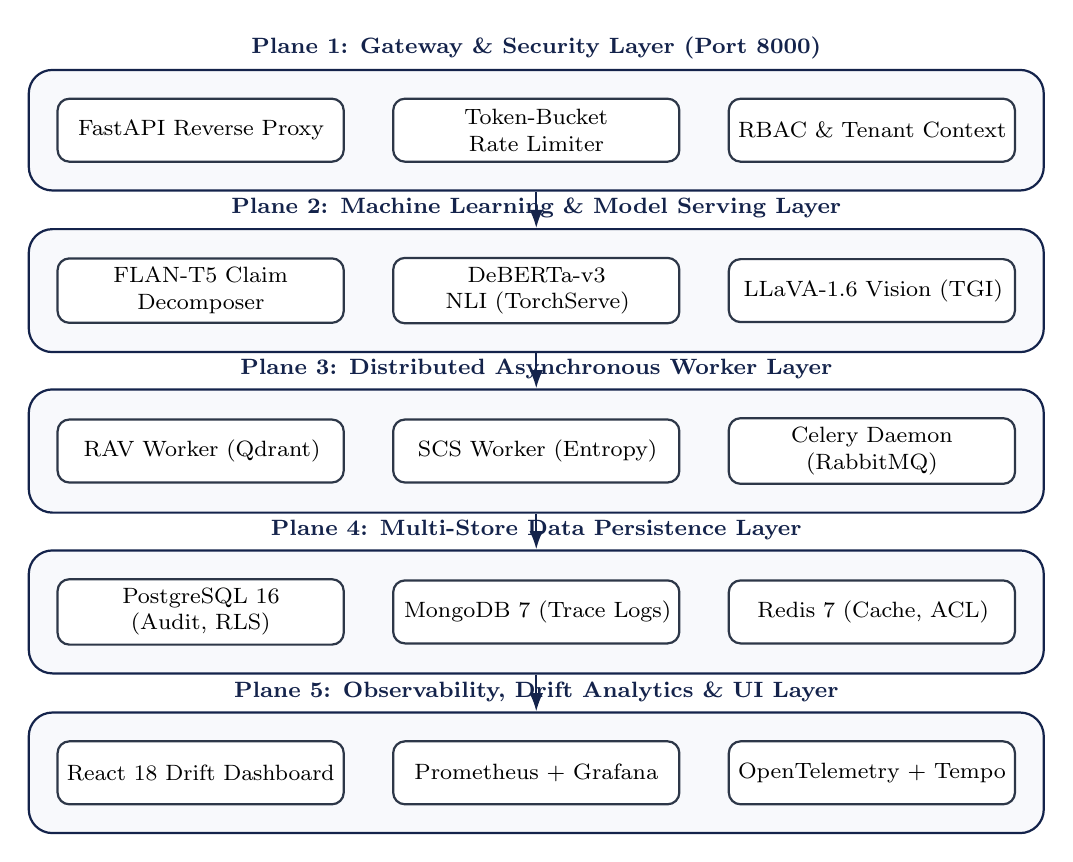
\begin{tikzpicture}[
    every node/.style={font=\footnotesize},
    plane/.style={rectangle, rounded corners=3mm, draw=primarynavy, thick, inner sep=10pt, fill=lightgreybg},
    cnode/.style={rectangle, rounded corners=1.5mm, draw=darkslate, fill=white, thick, text width=3.4cm, align=center, minimum height=0.8cm}
]

% Plane 1: Ingestion & Gateway
\node[cnode] (gw1) {FastAPI Reverse Proxy};
\node[cnode, right=0.6cm of gw1] (gw2) {Token-Bucket Rate Limiter};
\node[cnode, right=0.6cm of gw2] (gw3) {RBAC \& Tenant Context};
\begin{scope}[on background layer]
\node[plane, fit=(gw1)(gw2)(gw3), label=above:{\textbf{\color{primarynavy}Plane 1: Gateway \& Security Layer (Port 8000)}}] (p1) {};
\end{scope}

% Plane 2: Claim & ML Inference
\node[cnode, below=1.2cm of gw1] (ml1) {FLAN-T5 Claim Decomposer};
\node[cnode, right=0.6cm of ml1] (ml2) {DeBERTa-v3 NLI (TorchServe)};
\node[cnode, right=0.6cm of ml2] (ml3) {LLaVA-1.6 Vision (TGI)};
\begin{scope}[on background layer]
\node[plane, fit=(ml1)(ml2)(ml3), label=above:{\textbf{\color{primarynavy}Plane 2: Machine Learning \& Model Serving Layer}}] (p2) {};
\end{scope}

% Plane 3: Distributed Execution Workers
\node[cnode, below=1.2cm of ml1] (wk1) {RAV Worker (Qdrant)};
\node[cnode, right=0.6cm of wk1] (wk2) {SCS Worker (Entropy)};
\node[cnode, right=0.6cm of wk2] (wk3) {Celery Daemon (RabbitMQ)};
\begin{scope}[on background layer]
\node[plane, fit=(wk1)(wk2)(wk3), label=above:{\textbf{\color{primarynavy}Plane 3: Distributed Asynchronous Worker Layer}}] (p3) {};
\end{scope}

% Plane 4: Multi-Store Persistence
\node[cnode, below=1.2cm of wk1] (db1) {PostgreSQL 16 (Audit, RLS)};
\node[cnode, right=0.6cm of db1] (db2) {MongoDB 7 (Trace Logs)};
\node[cnode, right=0.6cm of db2] (db3) {Redis 7 (Cache, ACL)};
\begin{scope}[on background layer]
\node[plane, fit=(db1)(db2)(db3), label=above:{\textbf{\color{primarynavy}Plane 4: Multi-Store Data Persistence Layer}}] (p4) {};
\end{scope}

% Plane 5: Observability & Dashboard
\node[cnode, below=1.2cm of db1] (ob1) {React 18 Drift Dashboard};
\node[cnode, right=0.6cm of ob1] (ob2) {Prometheus + Grafana};
\node[cnode, right=0.6cm of ob2] (ob3) {OpenTelemetry + Tempo};
\begin{scope}[on background layer]
\node[plane, fit=(ob1)(ob2)(ob3), label=above:{\textbf{\color{primarynavy}Plane 5: Observability, Drift Analytics \& UI Layer}}] (p5) {};
\end{scope}

\draw[-Latex, thick, primarynavy] (p1) -- (p2);
\draw[-Latex, thick, primarynavy] (p2) -- (p3);
\draw[-Latex, thick, primarynavy] (p3) -- (p4);
\draw[-Latex, thick, primarynavy] (p4) -- (p5);

\end{tikzpicture}
\caption{The Five-Plane Architecture of the MIRAGE Enterprise Middleware.}
\label{fig:five_planes}
\end{figure}

\subsection{Low-Level Design \& Technical Stack}

\begin{table}[H]
\centering
\small
\renewcommand{\arraystretch}{1.25}
\begin{tabularx}{\linewidth}{p{3.5cm} p{4.2cm} X}
\toprule
\textbf{Component Layer} & \textbf{Technology Selected} & \textbf{Rationale \& Specification Guarantee} \\
\midrule
\textbf{API Gateway} & FastAPI (Python 3.12) & Async I/O, sub-10ms overhead, automated OpenAPI generation. \\
\textbf{Claim Decomposer} & Fine-tuned FLAN-T5-base & Pure CPU inference ($<50$ms), zero GPU dependency for extraction. \\
\textbf{NLI Model Server} & TorchServe (DeBERTa-v3) & FP16 GPU inference ($\sim 2$GB VRAM) with dynamic batching. \\
\textbf{Visual Model Server} & TGI (LLaVA-1.6-Mistral-7B) & 4-bit AWQ quantization ($\sim 14$GB VRAM) for multimodal VQA. \\
\textbf{Vector Database} & Qdrant v1.11 & HNSW indexing, per-tenant namespace isolation (\texttt{kb\_\{tenant\_id\}}). \\
\textbf{Task Broker} & RabbitMQ 3.13 Quorum & Disk-backed Raft consensus, late consumer acks, no message loss. \\
\textbf{Cache \& Rate Limit} & Redis 7.2 (ACL DB0 / DB1) & Microsecond Lua token-bucket rate limiting via \texttt{TIME} opcode. \\
\textbf{Relational Database} & PostgreSQL 16 & Row-Level Security (RLS), SHA-256 chained tamper-evident audit logs. \\
\textbf{Trace Persistence} & MongoDB 7.0 & Schema-flexible verification trace documents per tenant collection. \\
\textbf{Observability} & OTel Collector + Tempo & Distributed W3C trace context, zero prompt leakage in spans. \\
\bottomrule
\end{tabularx}
\caption{Production Technology Stack Breakdown and Architectural Rationale.}
\label{tab:tech_stack}
\end{table}

% ==============================================================================
% SECTION 7: COMPARATIVE ANALYSIS
% ==============================================================================
\section{Comparative Benchmark Analysis}

How does MIRAGE compare against existing academic and commercial baselines?

\begin{table}[H]
\centering
\small
\renewcommand{\arraystretch}{1.3}
\begin{tabularx}{\linewidth}{X c c c c c}
\toprule
\textbf{Feature / Capability} & \textbf{Raw LLM} & \textbf{SelfCheckGPT} & \textbf{FACTSCORE} & \textbf{LLM Judge} & \textbf{MIRAGE (Ours)} \\
\midrule
\textbf{Multi-Signal Verification} & No & No (SCS only) & No (RAG only) & No (Self-eval) & \textbf{Yes (5 Signals)} \\
\textbf{Multimodal (Image) Grounding} & No & No & No & Rare & \textbf{Yes (CLIP+LLaVA)} \\
\textbf{Calibrated Risk Probability} & No & No & No & No & \textbf{Yes ($ECE < 0.05$)} \\
\textbf{Conformal Coverage Bounds} & No & No & No & No & \textbf{Yes ($\ge 94\%$)} \\
\textbf{Feature Attribution (Explain)} & No & No & No & Vague & \textbf{Yes (TreeSHAP)} \\
\textbf{Self-Healing Correction Loop} & No & No & No & Unstable & \textbf{Yes (LangGraph)} \\
\textbf{Latency SLA ($P95$)} & Baseline & $>6$ sec & $>4$ sec & $>5$ sec & \textbf{$<3.0$ seconds} \\
\textbf{Zero Client Code Changes} & Yes & No & No & No & \textbf{Yes (Drop-in Proxy)} \\
\bottomrule
\end{tabularx}
\caption{Feature and Performance Comparison Between MIRAGE and State-of-the-Art Baselines.}
\label{tab:comparison}
\end{table}

% ==============================================================================
% SECTION 8: IMPLEMENTATION FEASIBILITY & TIMELINE
% ==============================================================================
\section{Hardware Budget, Feasibility and Project Timeline}

\subsection{Dual Deployment Profile (Zero-Cost Dev vs. Cloud Production)}
\begin{itemize}[leftmargin=*]
    \item \textbf{Academic / Zero-Cost Development Profile:} Built for student development without cloud bills. Uses Groq / OpenRouter free-tier LLM endpoints, local Docker Compose microservices, and CPU fallback for claim extraction and NLI.
    \item \textbf{Production Enterprise Cloud Profile:} Deployed on an AWS \texttt{g5.2xlarge} instance (NVIDIA A10G GPU, 24GB VRAM, 8 vCPUs, 32GB RAM).
    \begin{itemize}
        \item \textit{DeBERTa-v3-large (FP16):} $\sim 2.1$ GB VRAM.
        \item \textit{LLaVA-1.6-Mistral-7B (4-bit AWQ):} $\sim 14.2$ GB VRAM.
        \item \textit{KV Cache + Batching Headroom:} $\sim 7.7$ GB VRAM.
        \item \textit{Total VRAM Consumption:} $\sim 16.3$ GB / 24 GB ($68\%$ utilization, fully safe).
    \end{itemize}
\end{itemize}

\subsection{Current Project Progress and 6-Month Roadmap}
The MIRAGE project has successfully completed foundational infrastructure hardening (Phases P0.1 through P0.6) and is currently in active Phase P1 development:

\begin{table}[H]
\centering
\small
\renewcommand{\arraystretch}{1.25}
\begin{tabularx}{\linewidth}{p{2.8cm} p{3.2cm} X c}
\toprule
\textbf{Milestone} & \textbf{Target Schedule} & \textbf{Key Deliverables \& Verification Artifacts} & \textbf{Status} \\
\midrule
\textbf{Phase P0 (0.1--0.6)} & August--Sept 2026 & Cryptographic JWT/API Auth, Postgres RLS, Mongo Dual-Write, Redis Token-Bucket, RabbitMQ Quorum Queues, 13-Container Docker Compose Topology. (307/307 Automated Pytest Suite Passed). & \textbf{COMPLETED} \\
\textbf{Phase P1} & September 2026 & REST API Conformance (\texttt{/v1/sessions/\{id\}}, \texttt{/v1/alerts}, \texttt{/v1/reports/generate}, \texttt{/v1/reports/\{id\}/pdf}, \texttt{/v1/kb/upload}). & \textbf{IN PROGRESS} \\
\textbf{Phase P2} & October 2026 & React 18 Drift Dashboard, interactive SHAP waterfall views, WebSocket live streaming verification client. & \textbf{PLANNED} \\
\textbf{Phase P3} & November 2026 & k6 load testing (100 concurrent users at $P95 < 3$s) and Toxiproxy fault-injection chaos engineering. & \textbf{PLANNED} \\
\textbf{Phase P4} & December 2026 & Comprehensive benchmark evaluation across TruthfulQA, HaluEval, MMHAL-Bench, and FActScoring. & \textbf{PLANNED} \\
\textbf{Phase P5} & January 2027 & Research paper draft submission to AI Safety / NLP venue and final project defense. & \textbf{PLANNED} \\
\bottomrule
\end{tabularx}
\caption{MIRAGE Project Roadmap and Implementation Milestones.}
\label{tab:roadmap}
\end{table}

% ==============================================================================
% SECTION 9: CONCLUSION & APPROVAL SIGN-OFF
% ==============================================================================
\section{Conclusion and Faculty Approval Request}

Hallucination in Large Language Models is widely recognized as the single largest bottleneck preventing the safe adoption of generative AI in enterprise operations. The \textbf{MIRAGE} platform addresses this challenge not through superficial prompting or uncalibrated scoring, but through a mathematically grounded, multi-signal, and production-hardened microservices architecture.

With 307 passing automated regression tests, a ratified 13-service container topology, rigorous formal threat modeling, and a drop-in integration design, this project demonstrates high research novelty alongside industry-standard software engineering rigor.

\vspace{0.8cm}

\noindent We respectfully request the faculty review committee's formal approval to proceed with the remaining implementation phases and final evaluation.

\vspace{1.5cm}

\begin{minipage}[t]{0.45\textwidth}
    \rule{\linewidth}{0.6pt}\\
    \textbf{Vedant Panchal (23AIML042)}\\
    Student, Dept. of Artificial Intelligence \& ML\\
    Chandubhai S. Patel Institute of Technology
\end{minipage}
\hfill
\begin{minipage}[t]{0.45\textwidth}
    \rule{\linewidth}{0.6pt}\\
    \textbf{Dax Virani (23AIML076)}\\
    Student Investigator, B.Tech AIML\\
    Chandubhai S. Patel Institute of Technology
\end{minipage}

\vspace{1.5cm}

\begin{minipage}[t]{0.45\textwidth}
    \rule{\linewidth}{0.6pt}\\
    \textbf{Project Guide / Supervisor}\\
    Department of AI \& ML\\
    CSPIT, CHARUSAT
\end{minipage}
\hfill
\begin{minipage}[t]{0.45\textwidth}
    \rule{\linewidth}{0.6pt}\\
    \textbf{Head of Department (HOD)}\\
    Department of AI \& ML\\
    CSPIT, CHARUSAT
\end{minipage}

\end{document}
